%% LyX 2.1.3 created this file.  For more info, see http://www.lyx.org/.
%% Do not edit unless you really know what you are doing.
\documentclass[english]{article}
\usepackage{standalone}
\usepackage{times}
\usepackage[utf8]{luainputenc}
\usepackage{microtype}
\usepackage{geometry}
\geometry{verbose,tmargin=2.5cm,bmargin=2cm,lmargin=1.5cm,rmargin=1.5cm}
\usepackage{babel}
\usepackage{verbatim}

\usepackage{tikz}
\usetikzlibrary{positioning, fit,arrows,shapes.geometric}
\usetikzlibrary{backgrounds}
\usetikzlibrary{shadows}
\usepgflibrary{shadings}

\usepackage{xcolor}
\usepackage{pgfgantt}


\usepackage[backend=bibtex,
citestyle=verbose,
bibencoding=ascii,
maxcitenames=99,
url=true,
hyperref=true
]{biblatex}
\bibliography{master}
\DeclareFieldFormat{abstract}{\par Abstract: \emph{#1}}
\renewbibmacro*{finentry}{\printfield{abstract}\finentry}

\usepackage{cleveref}

\begin{document}

\title{Annual Report 2015-2016}
\author{Lyndon White}

\maketitle

\section{Summary of Research Progress to Date}

Work has proceeded, without significant deviation from Project Proposal. All this work has yielded publication, or is pending publication; so in the following sections, I will allow the publications abstracts to describe the work.


\subsection{Semantic Evaluation}
\begin{comment}

An investigation into the semantic constancy was carried out. 
The goal was to find out which methods for sentence embeddings were good
The definition of \emph{good }was made concrete as a specification on the relationship between 
the partitioning of sentence space by meaning,
and the corresponding areas of the vector sentence embedding space.
A good sentence embedding method would exhibit the following factors: All sentences with same meaning go to small area in vector space; The areas should not overlap, and should be separate; the areas should have no twists, bulges, holes, jumps etc.      			
It was noted that these are also the conditions for a classifier to work well.
So a classification task can was used to assess the quality of an embedding method.

For this classification to be done, required the sentences to be grouped into semantically equivalent classes.
This uses the formal definition of semantic equivalence. A pair of sentences are considered semantically equivalent of they exhibit bidirectional entailment.
That is to say, if one being true implies the other is true, and that the reverse also holds. By taking the transitive and symmetric closure of this equivalence relation,
the a set of equivelence classes can be found.\\
This was done to the Microsoft research paraphrase corpus, which contains pairs of paraphrases. 
Some sentences occurred in multiple paraphrase pairs.
Thus the closure yields paraphrase groups of suitable size for evaluation.

However there were very few large paraphrase groups. So for additional verification, a new corpus was constructed.
This was based on the Opinosis corpus of highly redundant product reviews. This required manual grouping.
The new corpus yielded much larger groups, and was more challenging as a evaluation task than the existing corpus.
Both corpora were made available online at: \url{http://white.ucc.asn.au/resources/paraphrase_grouped_corpora/}.

The surprising result was that the simple methods including bag of words, and the mean and sum of word embeddings performing significantly better than the more complex models. This added relevance to the next area of work.

\end{comment}

\subsubsection{Publications Arising}
This work was accepted into the 20th Australasian Document Computing Symposium (ADCS). Where it was presented as an oral, and as a poster to the combined session with  Australian Linguistic Society (ALS), the Australasian Language Technology Association (ALTA), and the Australian Music Psychology Society (AMPS Inc.).
\vspace{1cm}

\fullcite{White2015SentVecMeaning}


\subsection{Sentence Generation from Sum of Word Embeddings}
\begin{figure}[h!]
	\begin{center}
		\documentclass{standalone}

\usepackage{tikz}
\usetikzlibrary{positioning}


\begin{document}

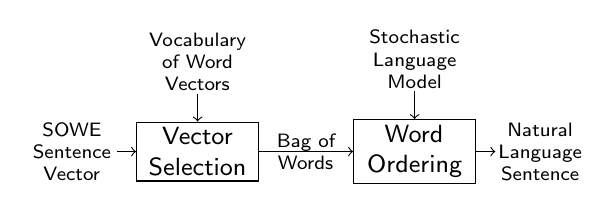
\begin{tikzpicture}[
	every node/.style={ text width=4em,
    					align=center,
                        font=\scriptsize\sffamily,
                        inner sep=1pt
                        },
	proc/.style= {draw,
    			  font=\small\sffamily,
                  inner sep = 2pt
    }
]
	\node (input) [inner sep=-4pt] {SOWE Sentence Vector};
    \node (selection) [proc, right = 0.7em of input]{Vector\\ Selection};
    \node (ordering) [proc, right = 3.4em of selection]{Word\\ Ordering};
	\node (vocab) [above = 1em of selection]{Vocabulary of Word Vectors};
    \node (lm) [above = 1em of ordering] {Stochastic Language Model};
    \node (output) [inner sep=-4pt, right=0.7em of ordering] {Natural Language Sentence};
    \draw[->] (input) -- (selection);
    \draw[->] (vocab) -- (selection);
    \draw[->] (selection) -- (ordering) node[midway] {Bag of Words};
    \draw[->] (lm) -- (ordering);
    \draw[->] (ordering) -- (output);
\end{tikzpicture}

\end{document}	
	\end{center}
	\caption{\label{fig:block} The two step process for generating sentences.}
\end{figure}



\subsubsection{Publications Arising}
This work was broken into two prepared publications, according to the two steps incolved in the process as shown in \Cref{fig:block}
This covers the first half of going from Sum of word embedding, to a bag of words as a conference paper.


\fullcite{White2015BOWgen}
\vspace{1cm}


The second publication, is currently in late stages editing, and is being prepared as a journal article. This covers the whole work, end to end on generating sentences from sums of word embeddings. This includes utilising the bag of words generation step, and adding the word ordering step.

\fullcite{SOWEgen}
\vspace{1cm}

This work was also presented orally to an informal half-day ``Workshop on Deep Learning for Natural Language Processing'', internally within UWA.


\subsection{Problems}
There have not been significant problems this year.
A minor problem was the lack of LDC resources.
LDC includes many of the standard corpora used for NLP. Access to LDC is on subscription, per calendar year and is several thousand dollars.
During that access period, the corpora can be obtained permanently without additional charge.
We chose to delay acquiring a subscription until the new year, that we might take a full year to select and acquire the most useful resources.
I believe this was the correct choice (and indeed it was at my suggestion). However ideally we would always have had an LDC subscription.
More recently other large resources have become publicly available, which allowed the previous work. 
However the data from LDC would have made it easier to perform additional validation and benchmarking.
We now have access to LDC.


\newpage

\section{Updated Project Plan}
As the thesis is by publication, the key progress indicator towards textual completion, in the publications. As mentioned above 1 publication has been completed, 1 submitted, and a third is in the final stages of editing. These will form key chapters in the thesis.

The Gnatt Chart showing in \Cref{gantt} is largely unchanged from the that in the project proposal. It shows the tasks remaining to be completed; and the tasks completed. 

One change is the removal of the "semisupervised semantics constraints" sr, to  be replaced with a "characteristic vector autoregression" task. This new task has additional clarity on the method being used. As part of the investigations with this method, semi-supervised semantic constraints may be included. Similarly Tree search has been replaced with Structure search -- this is merely a clarification that there may be non-tree structures that form the best representation of sentences.


\begin{figure}
	\resizebox{0.9\textwidth}{!}{\centering
		\documentclass{standalone}
\usepackage{tikz}
\usetikzlibrary{positioning, fit,arrows,shapes.geometric}
\usetikzlibrary{backgrounds}
\usetikzlibrary{shadows}
\usepgflibrary{shadings}

\usepackage{xcolor}
\usepackage{pgfgantt}

\begin{document}

\ganttset{
group/.append style={fill=none},
milestone/.append style={},
%
ms/.style={milestone left shift=0.8,
	milestone right shift=0.2,
	milestone/.append style={fill=purple}},
%
paper/.style={milestone left shift=1.9,
	milestone right shift=-0.9,
	milestone/.append style={violet, circle}},
%
halfslot/.style={milestone left shift=2.9},
}

\pgfdeclarelayer{background}
\pgfdeclarelayer{foreground}
\pgfsetlayers{background,main,foreground}

\tikzset{node distance=1.5ex}
\tikzset{ms/.style={circle, minimum height=11pt}}
\begin{ganttchart}[%Specs
     y unit title=0.5cm,
     y unit chart=1.1cm,
     x unit = 1.5cm,
     vgrid={
     	*2{draw=none}, *1{dotted}, *1{red, dashed}
     	},
     hgrid,
     title height=1,
%     title/.style={fill=none},
     title label font=\bfseries\footnotesize,
     bar/.style={fill=blue},
     bar height=0.7,
%   progress label text={},
%
     group right shift=0,
     group top shift=0.7,
     group height=.3,
     group peaks width={0.2},
     newline shortcut=true,
     bar label node/.append style={align=right},
     canvas/.append style={fill=none},
   	 today = 9,
   	 today rule/.append style={red},
   	 today label=Work Complete,
]
{2}{14}

\gantttitle{2015}{3} 
\gantttitle{2016}{4} 
\gantttitle{2017}{4}
\gantttitle{2018}{2}
\\
\foreach \ii in {1, ..., 3}{
	\gantttitle{Apr--Jun}{1}
	\gantttitle{Jul--Sep}{1}
	\gantttitle{Oct--Dec}{1}
	\gantttitle{Jan--Mar}{1}
}
\gantttitle{Apr--Jun}{1}



\ganttgroup{Preparation}{2}{3} \\
\ganttbar{Review of\\ Literature}{2}{3}
\ganttbar[bar top shift=0.6pt, bar height=0.1pt, bar/.append style={fill=blue!20,}]{}{4}{12}\\
\ganttbar{Determine Focus\\ of Research}{2}{2} \\
\ganttbar{Investigate/Implement\\ Current Methods}{2}{2} \\


\ganttgroup{Research Tasks}{0}{0} \\
\ganttset{bar/.append style={fill=green!90!black}}
\ganttbar{Semantic\\ Evaluation}{3}{3} 
\ganttmilestone[paper, inline]{}{3}
\\
\ganttbar{Sum of Word\\ Embeddings}{4}{5}
\ganttmilestone[paper, halfslot,inline]{}{4}
\ganttmilestone[paper,inline]{}{5}
 \\
 \ganttbar{Word-Sense \\ Embeddings}{6}{7} 
\ganttmilestone[paper]{}{7}
\\
\ganttbar{Meaning\\ of Water}{8}{8} 
\\

\ganttbar{Color\\ Description}{9}{10} 
\ganttmilestone[paper]{}{10}

\\


\ganttbar{Structured\\ Models}{11}{12}
\ganttmilestone[paper]{}{12}
\ganttmilestone[paper]{}{11}
 \\


\ganttgroup{Milestones}{0}{0} \\
\ganttset{bar/.append style={fill=purple}}
\ganttmilestone[ms]{Research Proposal}{3}\\
\ganttmilestone[ms]{Annual Reports}{5}
\ganttmilestone[ms]{}{9}\\
\ganttbar{Dissertation \\Compilation}{13}{14}\\
\ganttmilestone[ms]{Submission}{14}

\begin{pgfonlayer}{foreground}
	\node(legend) at ([yshift=-100pt, xshift=-120pt]current bounding box.north east){Key:};
	\node(milestone)[below = 2ex of legend.west,ms, fill=purple, shape=diamond]{};
	\node[right = of milestone]{Milestone};
	\node(paper)[below = of milestone, ms, fill=violet] {};

	\node(lbl_paper)[right = of paper]{Paper Draft};
 \end{pgfonlayer}

\begin{pgfonlayer}{main}
	\node[drop shadow, fill=white, rounded corners=1pt, draw, fit = (legend) (lbl_paper)(paper)] {};
 \end{pgfonlayer}
\end{ganttchart}


\end{document}

	}
	\caption{\label{gantt} an Updated Gnatt Chart}
\end{figure}




\end{document}
